\section{Zielsetzung}
Ziel dieses Versuchs ist es den Absorptionskoeffizienten von verschiedener Materialien zu bestimmen.
Dafür wird die Wechselwirkung von $\gamma$- und $\beta$-Strahlung mit diesen Materialien untersucht.
\section{Theorie}
\label{sec:Theorie}
\subsection{Absorption}
Trifft ein Teilchenstrahl auf Materie, so finden Wechselwirkungen mit dieser statt.
Der Wirkungsquerschnitt $\sigma$ stellt ein Maß für die Häufigkeit der Wechselwirkungen dar.
Die Wahrscheinlichkeit, dass ein Teilchen eine Reaktion auslöst beträgt für einen Absorber mit Querschnitt F und Dicke D:
\begin{equation}
  W= \frac{nFD\sigma}{F}= nD \sigma
\end{equation}
Wenn $N_0$ Teilchen auf den Absorber treffen, finden
\begin{equation}
  N = N_0 nD \sigma
  \label{eq:gl1}
\end{equation}
Wechelwirkungen pro Zeit statt.
Bei einem realen Absorber muss, aufgrund der Vielzahl der Atome pro Volumeneinheit, $\sigma$ über eine infinitesimal dünne Schicht $dx$ aufsummiert werden.
Es kann nicht davon ausgegangen werden, dass die $\sigma$ sich in Strahlrichtung nicht überdecken.
Es wird angenommen, dass diese dünne Schicht $dx$ an einer Stelle $x$ innerhalb des Absorbers, mit der Dicke D, befindet.
Dann finden gemäß Gleichung \eqref{eq:gl1}
\begin{equation}
  dN = -N(x) n \sigma dx
\end{equation}
Reaktionen statt.
Die Zahl der Teilchen, welche nach Durchgang durch den Absorber übrigbleiben, lässt sich durch Integration über alle Schichten dx finden.
Damit ergibt sich die Gleichung:
\begin{equation}
  N(D) = N_0 \exp(-n\sigma D)
\end{equation}
Diese ist streng gültig, wenn jedes einfallende Teilchen höchstens eine Wechselwirkung mit der Materie eingeht.
Der Exponentialfaktor,
\begin{equation}
  \mu = n \sigma   ,
\end{equation}
wird als Absorbtionskoeffizient bezeichnet.
Es wird angenommen, dass die Elektronen eines Absorbermaterials die Wechselwirkungszentren darstellen.
Es folgt:
\begin{equation}
  n= \frac{z N_L \rho}{M}
  \label{eq:gl2}
\end{equation}
Hier ist $N_L=2.68\cdot 10^{25} m^-3$\cite{Nl} die Loschmidtsche Zahl, welche die Anzahl der Molekühle pro Volumeneinheit eines idealen Gases angibt, und $M$ das Molekulargewicht.
Aus Gleichung \eqref{eq:gl2} folgt für den Wirkungsquerschnitt:
\begin{equation}
  \sigma=\frac{\mu M}{z N_L \rho}
  \label{eq:wirk}
\end{equation}
Gleichung \eqref{eq:wirk} ist eine grobe Näherung der Realität.
\subsection{\texorpdfstring{$\gamma$}{Gamma}-Strahlung}
Atomkerne besitzen diskrete Energieniveaus.
Wenn ein Atomkern in einen energetisch niedrigen Zustand übergeht, so wird $\gamma$-Strahlung emittiert.
Diese weist Eigenschaften einer elektromagnetischen Welle auf, so kann die Energie der $\gamma$-Strahlung
nach der Quantenmechanik wie folgt angegeben werden:
\begin{equation}
  E_\gamma = h\nu
\end{equation}
Hier ist $h$ das Planksche Wirkungsquantum ($h=\SI{6.26e-34}{\joule\second}$\cite{planck}).
Die $\gamma$-Strahlung kann beim Eindringen in eine Materieschicht mit den Atomelektronen, den Kernen und ihren elektrischen Feldern eine Vielzahl von Wechselwirkungen eingehen.
In diesem Versuch sind die wichtigsten Wechselwirkunsprozesse der Photo-Effekt, der Compton-Effekt und die Paarbildung.
Bei dem Photo-Effekt wechselwirkt ein $\gamma$-Quant mit einem Hüllenelektron, dabei wird das $\gamma$-Quant vernichtet und das Elektron aus seiner Bindung entfernt.
Die kinetische Energie des Elektrons lässt sich dann mit
\begin{equation}
  E_e = h\nu - E_B
\end{equation}
angeben.
$E_B$ stellt die Bindungsenergie des Elektrons dar.
Das Auftreten des Photoeffekts ist also nur möglich wenn $h\nu > E_B$ gilt.
Durch den Impulssatz folgt, dass das Atom einen Teil des Quantenimulses aufnehmen muss.
Dies ist nur wahrscheinlich, wenn das Elektron möglichst fest an das Atom gebunden ist.
Daraus folgt, dass das Auftreten des Photoeffekts unwahrscheinlicher wird, wenn $E_\gamma$  viel größer als die Bindungsenergie ist.


Der zweite zu betrachtende Effekt ist der Comptoneffekt.
Dieser beschreibt die Streuung an einem freien Elektron.
Es kommt zu einer Richtungs- und Energieänderung.
Das $\gamma$-Quant kann nach Energie- und Impulssatz nicht seine komplette Energie an ein freies Elektron abgeben.
Es wird also nach der Wechselwirkung nicht annihiliert.
Die Intensität des $\gamma$-Strahls nimmt ab.
Der Wirkungsquerschnitt lässt sich nach Nischina und Klein mit
\begin{equation}
    \label{eq:klein}
  \sigma_{Com} = 2 \pi r_e^2 \left\{\frac{1+\varepsilon}{\varepsilon^2}\left[\frac{2(1+\varepsilon)}{1+2\varepsilon} - \frac{1}{\varepsilon}ln(1+2\varepsilon)\right] + \frac{1}{2\varepsilon}ln(1+2\varepsilon) - \frac{1+3\varepsilon}{(1+2\varepsilon)^2} \right\}
\end{equation}
berechen.
Das Verhältnis der Quantenergie $E_\gamma$ zur Ruheenergie des Elektrons wird durch
\begin{equation}
  \varepsilon = \frac{E_\gamma}{m_0 c^2}
\end{equation}
ausgedrückt und
\begin{equation}
  r_e= 2.82 \cdot 10^-15 \si{\meter}
\end{equation}
bezeichet den "klassischen Elektronenradius".
Es soll nicht angedeutet werden, dass ein Elektron einen endlichen Radius besitzt, sondern die Streuwahrscheinlichkeit angegeben werden.
Bei der Betrachtung von $\sigma_{Com}$ für kleine Energien lässt sich feststellen, dass $\sigma_{Com}$ nahezu Energieunabhängig ist und gegen den Thomsonschen Wirkungsquerschnitt strebt:
\begin{equation}
  \lim_{\varepsilon \rightarrow 0} \sigma_{Com}(\varepsilon) = \frac{4}{3} \cdot 2 \pi r_e^2 = \frac{8}{3}\pi r_e^2 =: \sigma_{Th}
\end{equation}
Die Paarbildung tritt ein, wenn die $\gamma$-Energie größer als die doppelte Ruheenergie des Elektrons ist.
Dann wird das $\gamma$-Quant unter Bildung eines Elektrons und eines Positrons annihiliert.
Es ist nicht ausreichend das die Energie des erwähnten Betrages absorbiert wird, sondern es benötigt einen zusätzlichen Stoßpartner.
Dazu dienen meistens Atomkerne des Absorbermaterials.
\subsection{\texorpdfstring{$\beta$}{Beta}-Strahlung}
Ein Atomkern mit instabiler Anordnung von Protonen- oder Neutronenzahl emittiert positiv oder negativ geladene Elektronen hoher kinetischer Energie.
Die $\beta$-Teilchen entstehen nach einer der folgenden Gleichungen:
\begin{eqnarray}
n \rightarrow p + \beta^- + \bar{\nu_e} \\
\nonumber
\text{oder}\\
p \rightarrow n + \beta^+ + \nu_e 
\end{eqnarray}
Neben dem Elektron wird ein weiteres Elementarteilchen emittiert.
Das Neutrino bzw. Antineutrino besitzt keine Ladung, eine sehr geringe Ruhemasse und geht mit der Materie nur schwache Wechselwirkungen ein.
Für die Wechselwirkung von $\beta$-Teilchen mit Materie ist ihre Ladung und im Vergleich zu anderen Teilchen geringe Masse von Bedeutung.
Diese führen dazu, dass $\beta$-Teilchen eine Vielzahl von Wechselwirkungsprozessen beim Durchgang durch Materie eingehen.
Die $\beta$-Absorption ist ein wesentlich komplexerer Vorgang als die Absorption der $\gamma$-Strahlung.
%Es lässt sich zeigen, dass für $\beta$-Strahlung natürlicher Quellen, Gleichung für nicht zu große Schichtdicken gültig ist.
\begin{figure}[H]
    \centering
    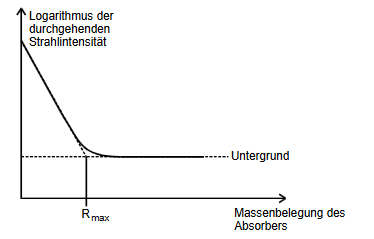
\includegraphics[scale=0.7]{content/Absorbbeta.png}
    \caption{Absorptionskurve eines natürlichen $\beta$-Strahlers.}
    \label{fig:abs}
\end{figure}
\noindent
In Abbildung \ref{fig:abs} ist eine typische Absorptionskurve eines natürlichen $\beta$-Strahlers dargestellst.
Anstelle der Schichtdicke D wurde die Massenbelgung
\begin{equation}
  R = \rho D
\end{equation}
verwendet.
Da die maximale Reichweite $R_{max}$ hauptsächlich durch die energiereichsten Elektronen bestimmt ist, kann aus dieser die beim $\beta$-Zerfall freiwerdende Gesamtenergie,
\begin{equation}
  E_{max}= 1.92  \sqrt{R_{max}^2 +0.22R_{max}} [\si{\mega e\volt}]
\end{equation}
bestimmt werden.
Aufgrund der Komplexität der Wechselwirkungsprozesse der $\beta$-Teilchen mit Materie existieren nur empirisch bestimmte Zusammenhänge zwischen den Größen $R_{max}$ und $E_{max}$.
